\chapter{Introdução}

\blindtext[2]

\section{Preliminares}

\blindtext[2]

\subsection{Motivação}

\blindtext[1]

\begin{figure}[H]
    \centering
    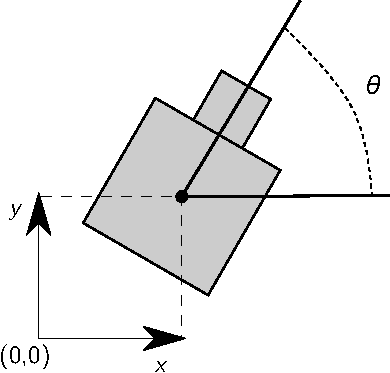
\includegraphics{figures/uav_localization.pdf}
    \caption[Nome da figura]{Nome da figura. Descrição da figura. Fonte: alguém}
\end{figure}

\blindtext[1]

\subsubsection{Atualidade}

\blindmathpaper

Uma função quadrática tem a seguinte forma \(f(x) = ax^2+bx+c\), com \(a,b,c \in \mathbb{R}\). Já a relação fundamental da trigonometria é \(\sin^2x+\cos^2x = 1\).

1234567890

\(1234567890\)